\selectlanguage{greek}
\chapter{Το πρόβλημα της Προσομοίωσης Κυκλωμάτων}
\label{ch:2.chapterCircuitSimulationPrinciples}
    
\section{Βασικές έννοιες ηλεκτρικών κυκλωμάτων}

\subsection{Γραμμικά κυκλώματα}

Ο πρώτος ορισμός που πρέπει να δώσουμε είναι αυτός του ηλεκτρικού κυκλώματος. Το ηλεκτρικό κύκλωμα αποτελεί ένα κλειστό δίκτυο συνδεδεμένων μεταξύ τους ηλεκτρικών στοιχείων εντός του οποίου υπάρχουν διαδρομές ρεύματος.

Το κάθε στοιχείο περιγράφεται από μια σχέση ρεύματος και τάσης. Για παράδειγμα, ένας πυκνωτής περιγράφεται από την συνάρτηση (με βάση τον νόμο του \textlatin{Ohm}) $u = Ri$.

\begin{figure}
    \centering
    \begin{minipage}{0.45\textwidth}
        \centering
        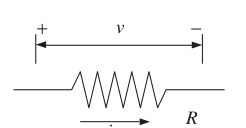
\includegraphics[width=0.9\textwidth]{Resistor}
        \caption{Στοιχείο αντίστασης}
    \end{minipage}\hfill
    \begin{minipage}{0.45\textwidth}
        \centering
        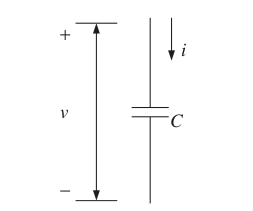
\includegraphics[width=0.9\textwidth]{Capacitor}
        \caption{Στοιχείο πυκνωτή}
    \end{minipage}
\end{figure}


Οι συναρτήσεις των στοιχείων ενός ηλεκτρικού κυκλώματος καθορίζουν αν το κύκλωμα θα είναι γραμμικό ή μη γραμμικό. Γραμμικό στοιχείο είναι το στοιχείο του οποίου η συνάρτηση δεν περιλαμβάνει συντελεστές στη δύναμη του 2 ή μεγαλύτερη.
Όταν ένα ηλεκτρικό κύκλωμα περιλαμβάνει μόνο στοιχεία γραμμικά τότε και το ίδιο το κύκλωμα είναι γραμμικό.

Στα πλαίσια της εργασίας, θα ασχοληθούμε αυστηρά μόνο με γραμμικά κυκλώματα τα οποία ακολουθούν την αρχή της επαλληλίας (\textlatin{superposition principle}).  Έτσι, η έξοδος ενός κυκλώματος $F(x)$,όταν εφαρμόζεται ένας γραμμικός συνδυασμός σημάτων $a_1x_1(t) + a_2x_2(t)$ ως είσοδος, θα ισούται με τον γραμμικό συνδυασμό των εξόδων των σημάτων $x_1(t)$ και $x_2(t)$ όταν αυτά εφαρμόζονται ξεχωριστά, δηλαδή:

\begin{equation}
    F\{a_1x_1(t) + a_2x_2(t)\} = a_1F\{x_1(t)\} + a_2F\{x_2(t)\}
\end{equation}


\subsection{Κυκλωματικά στοιχεία}

Με τον όρο κυκλωματικό στοιχείο στα πλαίσια της εργασίας μας, περιγράφουμε ηλεκτρικά στοιχεία με δύο τερματικά. Σαν γενικές κατηγορίες των στοιχείων αυτών έχουμε τα παθητικά και τα ενεργά στοιχεία. Τα ενεργά στοιχεία είναι αυτά που παρέχουν ηλεκτρική ενέργεια και δρουν ως πηγές ενός κυκλώματος. Οι πηγές που θα συναντήσουμε είναι ανεξάρτητες και έχουν την ιδιότητα ότι η τάση $v(t)$ ή το ρεύμα $i(t)$ που περνάει απο μέσα τους εκφράζεται ως εξής:
\begin{itemize}
    \item Ανεξάρτητη πηγή τάσης ορίζεται η πηγή της οποίας η τάση είτε είναι σταθερή ή μεταβάλλεται σε συνάρτηση με τον χρόνο $v = f(t)$. 
    \item Ανεξάρτητη πηγή ρεύματος ορίζεται η πηγή της οποίας το ρεύμα είτε είναι σταθερό ή μεταβάλλεται σε συνάρτηση με τον χρόνο $i = f(t)$.
\end{itemize}

Αντίθετα με τα ενεργά στοιχεία, τα παθητικά στοιχεία καταναλώνουν και δεν παράγουν ενέργεια. Η ενέργεια που καταναλώνουν τα παθητικά στοιχεία είτε θα μετατραπεί σε κάποιου άλλου είδους ενέργειας (για παράδειγμα θερμότητα) είτε θα αποθηκευτεί (σε ενέργεια ηλεκτρικού ή μαγνητικού πεδίου). Τονίζουμε ότι κατά την μετατροπή της ενέργειας, η ισχύς που υπολογίζουμε στην έξοδο δεν θα ενισχυθεί. Τα πιο γνωστά παθητικά στοιχεία είναι το πηνίο, η αντίσταση και ο πυκνωτής.

Αν δούμε τη μορφή της εξίσωσης που χαρακτηρίζει το κάθε στοιχείο μπορούμε να διαφοροποιήσουμε την κατηγοριοποίηση σε δύο ομάδες. Για αριθμό στοιχείων $m_1$ έχουμε την πρώτη ομάδα που έχει την παρακάτω μορφή εξίσωσης:

\begin{equation}
    i_k(t) = g_k u_k(t) + c_k \frac{du_k(t)}{dt} + s_k(t)
\end{equation}

Στην ομάδα αυτή έχουμε αντιστάτες, πυκνωτές και πηγές ρεύματος.

Αντίστοιχα, η δεύτερη ομάδα με αριθμό στοιχείων $m_2$ εκφράζεται από την παρακάτω μορφή εξίσωσης:

\begin{equation}
    u_k(t) = l \frac{\overrightarrow{d i_k}(t)}{dt} + \overrightarrow{s_k}(t)
\end{equation}

Στην δεύτερη ομάδα έχουμε πηνία και πηγές τάσης.

\subsection{Τροποποιημένη ανάλυση κόμβων}

Η συμπεριφορά ενός κυκλώματος περιγράφεται από ένα σύνολο εξισώσεων που σχηματίζεται συνδυάζοντας τις συναρτήσεις που προκύπτουν από τους νόμους του $Kirchoff$ για την τάση (\textlatin{Kirchoff's Voltage Law (KVL)} και το ρεύμα (\textlatin{Kirchoff's Current Law (KCL))}. Ορίζουμε τους παραπάνω νόμους ως εξής:

\begin{enumerate}
  \item Ο νόμος ρευμάτων του \textlatin{Kirchoff (KCL)}  μας λέει οτι το αλγεβρικό άθροισμα των ρευμάτων σε κάθε κόμβο ενός κυκλώματος ισούται με το μηδέν.
  \begin{equation}
    \label{4} \sum_{k=1}^{n}i_k(t) = 0 \Leftrightarrow A \overrightarrow{i}(t) = \overrightarrow{0}
  \end{equation}
  \item Ο νόμος τάσεων του \textlatin{Kirchoff(KVL)} μας λέει ότι σε κάθε κλειστό βρόγχο ενός κυκλώματος, το άθροισμα των τάσεων (διαφορών δυναμικού) των επιμέρους κλάδων που απαρτίζουν τον βρόγχο ισούται με το μηδέν.
  \begin{equation}
      \sum_{k=1}^{m}u_k(t) = 0 \Leftrightarrow \overrightarrow{u}(t) = A^T \overrightarrow{u}(t)
  \end{equation}
\end{enumerate}


Χρησιμοποιώντας τις συναρτήσεις που προκύπτουν από τους παραπάνω νόμους και ακολουθώντας τις κλασσικές μεθοδολογίες επίλυσης γραμμικών συστημάτων μπορούμε να βρούμε τη λύση για πολύ απλά συστήματα. Καταλαβαίνουμε όμως, με την κλασσική επίλυση των συστημάτων δεν μπορούμε να έχουμε κλιμάκωση στο μέγεθος των ηλεκτρικών κυκλωμάτων.

Για τον παραπάνω λόγο, μπορούμε να χρησιμοποιήσουμε την Τροποποιημένη Ανάλυση Κόμβων (\textlatin{Modified Nodal Analysis (MNA)}) για να λύσουμε με συστηματικό τρόπο συστήματα πολύ μεγάλης κλίμακας.

Τα βασικά βήματα για την Τροποποιημένη Ανάλυση Κόμβων είναι τα εξής:

\begin{enumerate}
    \item Γράφουμε με βάση τον Νόμο Ρεύματος του \textlatin{Kirchoff} την εξίσωση $Ai=0$ όπου $A$ είναι ο πίνακας μειωμένης πρόσπτωσης (\textlatin{reduced incidence matrix}) και το $i$ είναι διάνυσμα με όλα τα ρεύματα σε κάθε κλάδο
    \item Χρησιμοποιώντας τις εξισώσεις που περιγράφουν το κάθε κυκλωματικό στοιχείο, προσπαθούμε να εξαλείψουμε όσο το δυνατόν περισσότερες μεταβλητές ρεύματος με τη βοήθεια του Νόμου \textlatin{Kirchoff} για το ρεύμα. Με το βήμα αυτό καταλήγουμε να έχουμε εξισώσεις οι οποίες είναι σε συνάρτηση με την τάση $u = A^T v$.
    \item Στο βήμα αυτό, χρησιμοποιούμε τον Νόμο \textlatin{Kirchoff} για την τάση (\textlatin{Kirchoff's Voltage Law (KVL)}) και αντικαθιστούμε όλα τις τάσεις κλάδων με τάσεις κόμβων στη γείωση.
    \item Οι εξισώσεις στοιχείων των οποίων οι μεταβλητές τάσης δεν μπορούσαν να εξαλειφθούν, τις προσθέτουμε σαν επιπλέον εξισώσεις στο \textlatin{MNA} σύστημα.
\end{enumerate}

Με βάση τα παραπάνω βήματα καταλήγουμε στο εξής σύστημα ~\cite{ho1975modified}:
\begin{equation}
    \begin{bmatrix}
    Y & B\\
    C & Z
    \end{bmatrix}
    \begin{bmatrix}
    v\\
    i
    \end{bmatrix} = 
    \begin{bmatrix}
    s_v\\
    s_j
    \end{bmatrix}
\end{equation}


Όπου ισχύει η εξίσωση $Z_i + Y_u = s$ για $Z$ και $Y$ πίνακες ενώ $s$ είναι διάνυσμα.

% Οι παραπάνω εξισώσεις αφορούν αντίστοιχα τα στοιχεία των ομάδων 1 και 2.  ́Ετσι λοπόν
% προκύπτουν οι αντίστοιχες εξισώσεις:
% \begin{equation} \label{u1t}
%     \overrightarrow{u_1}(t) =  A^{T}_{1} \overrightarrow{u}(t)
% \end{equation}

% \begin{equation} \label{u2t}
%     \overrightarrow{u_2}(t) =  A^{T}_{2} \overrightarrow{u}(t)
% \end{equation}

% Αντίστοιχα, τώρα για τα στοιχεία των ομάδων 1 και 2, γράφουμε τις χακτηριστικές υπό την
% μορφή πινάκων:

% \begin{equation} \label{i1t}
%     \overrightarrow{i_1}(t) =  G \overrightarrow{u_1}(t) + C \frac{d \overrightarrow{u_1}(t)}{dt} + \overrightarrow{s_1}(t)
% \end{equation}

% \begin{equation} \label{u2t2}
%     \overrightarrow{u_2}(t) =  L \frac{d\overrightarrow{i_2}(t)}{dt} + \overrightarrow{s_2}(t)
% \end{equation}

% Επόμενο βήμα είναι η αντικατάσταση της εξίσωση \ref{u1t} στην εξίσωση \ref{i1t} και αντίστοιχα της εξίσωσης \ref{u2t} στην εξίσωση \ref{u2t2}. Μετά την αντίκατασταση προκύπτουν οι ακόλουθες εξισώσεις:

% \begin{equation} \label{A1GA}
%     A_1 G A^{T}_{1} \overrightarrow{u_1}(t) + A_1 C A^{T}_{1} \frac{d \overrightarrow{u_1}(t)}{dt} + A_2 \overrightarrow{i_2}(t) = - A_1 \overrightarrow{s_1} (t)
% \end{equation}

% \begin{equation} \label{AT2}
%     A^{T}_{2} \overrightarrow{u}(t) - L \frac{d \overrightarrow{i_1}(t)}{dt} = \overrightarrow{s_2}(t)
% \end{equation}

% Ο συνδυασμός των εξισώσεων \ref{A1GA} και \ref{AT2} δίνει ένα επεκταμένο (σύνθετο) σύστημα εξισώσεων διαστάσεων $[(n − 1) + m 2 ] × [(n − 1) + m 2 ]$, το οποίο το γράφουμε σε έναν ως εξής:
% \begin{center}
% \begin{bmatrix}
% A_1 G A^{T}_{1} & A_2\\
% A^{T}_{2} & 0
% \end{bmatrix} \begin{bmatrix}
% \overrightarrow{u_1}(t) \\
% \overrightarrow{i_2}(t)
% \end{bmatrix} + \begin{bmatrix}
% A_1 C A^{T}_{1} & 0\\
% 0 & -L
% \end{bmatrix} $\frac{d}{dt}$
% \begin{bmatrix}
% \overrightarrow{u_1}(t) \\
% \overrightarrow{i_2}(t)
% \end{bmatrix} = \begin{bmatrix}
% -A_1 \overrightarrow{s_1}(t) \\
% \overrightarrow{s_2}(t)
% \end{bmatrix}
% \end{center}


% Θέτοντας του πίνακες και τα διανύσματα ως:

% \begin{center}
% \widetilde{G} = \begin{bmatrix}
% A_1 G A_{1}^T & A_2 \\
% A_{2}^{T} & 0
% \end{bmatrix}, \widetilde{C} = \begin{bmatrix}
% A_1 C A_{1}^T & 0 \\
% 0 & -L
% \end{bmatrix}, \overrightarrow{x}(t) = \begin{bmatrix}
% \overrightarrow{u_1}(t) \\
% \overrightarrow{i_2}(t)
% \end{bmatrix}, \overrightarrow{e}(t) = \begin{bmatrix}
% -A_1\overrightarrow{s_1}(t) \\
% \overrightarrow{s_2}(t)
% \end{bmatrix}, 
% \end{center}

% λαμβάνουμε λαμβάνουμε τελικά, σε μια πιο ευδιάκριτη μορφή, ένα σύστημα γραμμικών διαφορικών εξισώσεων πρώτης τάξης με σταθερούς συντελεστές:

\begin{equation} \label{GxtCdxt}
\widetilde{G} \overrightarrow{x}(t) + \widetilde{C}\frac{d \overrightarrow{x}(t)}{dt} = \overrightarrow{e}(t) \Leftrightarrow \widetilde{G} \overrightarrow{x}(t) + \widetilde{C}\overrightarrow{x}(t) = \overrightarrow{e}(t)
\end{equation}

\section{Μεταβατική ανάλυση και ανάλυση συνεχούς}
Τα κυκλώματα στην πλειονότητα τους εκτός απο ανιστάτες περιλαμβάνουν και δυναμικά στοιχεία (πυκνωτές και πηνεία) τα οποία ανάλογα με τον χρόνο παρουσιάζουν μεταβολή.

Με βάση την παραπάνω παρατήρηση, η ανάλυση μας μπορεί με βάση τον χρόνο να οριστεί σε δυο κατηγορίες:
\begin{itemize}
    \item Ανάλυση συνεχούς: Σε αυτή την ανάλυση προσεγγίζουμε μια λύση του κυκλώματος για μια δεδομένη χρονική στιγμή.
    \item Μεταβατική ανάλυση: Αναφέρεται σε κυκλώματα με δυναμικά στοιχεία στα οποία μας ενδιαφέρει η απόκριση με βάση τον χρόνο.
\end{itemize}

\subsection{Ανάλυση συνεχούς}
Η παρούσα ανάλυση όπως τονίσαμε αναφέρεται σε συγκεκριμένες χρονικές στιγμές. Συνεπώς, υπολογίζουμε για διάφορα \textlatin{DC} σήματα την απόκριση που παρουσιάζει το κύκλωμα. Το χαρακτηριστικό της ανάλυσης είναι οτι λόγω της μη μεταβολής του χρόνου, έχουμε μηδενική χρονική παράγωγο για τις διεγέρσεις και τις αποκρίσεις.

Το σύστημα της εξίσωσης \ref{GxtCdxt} γίνεται:

\begin{equation}
    \begin{bmatrix}
        A_1 G A_1^T & A_2 \\
        A_2^T & 0
    \end{bmatrix}
    \begin{bmatrix}
        \overrightarrow{u_1} \\
        \overrightarrow{i_2}
    \end{bmatrix} = 
    \begin{bmatrix}
        -A_1 \overrightarrow{s_1} \\
        \overrightarrow{s_2}
    \end{bmatrix}
\end{equation}

Για την παραπάνω ανάλυση είναι σημαντικό να αναφερθούμε στους συμμετρικούς και θετικά ορισμένους πίνακες \textlatin{Symmetric and Positive Definite(SPD)} οι οποίοι παρουσιάζουν ιδιαίτερες ιδιότητες που μας βοηθούν για ταχύτερη επίλυση των συστημάτων. Για να προκύψουν τέτοιοι πίνακες είναι απαραίτητο το κύκλωμα να αποτελείται μόνο απο αντιστάσεις, πυκνωτές και πηγές ρεύματος. Όλα τα υπόλοιπα στοιχεία πρέπει να απουσιάζουν.

H συμμετρία \textlatin{symmetric} ενός πίνακα $A$ ορίζεται όταν ο πίνακας ισούται με τον αντίστροφο του, δηλαδή ισχύει $A(i, j) = A(j, i)$ για $i \neq j$.

\begin{equation}
A = A^T \Leftrightarrow A\ is\ symmetric, \forall A \in \mathbb{R} ^{nxn}
\end{equation}

Για την ιδιότητα του θετικά ορισμένου \textlatin{(positive definite)} πίνακα Α, είναι όταν η τετραγωνική μορφή είναι θετική για κάθε διάνυσμα εκτός του μηδενικού:

\begin{equation}
\overrightarrow{x}^T A \overrightarrow{x} > 0, \forall \overrightarrow{x} \in \mathbb{R}^{n}, \overrightarrow{x} \neq
 \overrightarrow{0} \Leftrightarrow A \ is \ positive\ definite
 \end{equation}

\subsection{Μεταβατική ανάλυση}

Αντίθετα με την ανάλυση συνεχούς (\textlatin{DC analysis}) όπου πραγματοποιείται η ανάλυση για συγκεκριμένες χρονικές στιγμές, στην μεταβατική ανάλυση \textlatin{Transient analysis} βασιζόμαστε στον υπολογισμό της χρονικής απόκρισης του κυκλώματος για δεδομένες διεγέρσεις.


Αρχικά αναζητούμε επίλυση για το πρόβλημα των αρχικών τιμών στο οποίο για δεδομένο διάνυσμα διεγέρσεων ${e}(t)$ και θεωρώντας πως το διάνυσμα των αποκρίσεων ${x}(t)$ είναι καθορισμένο για μία δεδομένη χρονική στιγμή $t_0$ ως ${x}(t_0)$ = ${x_0}$ (αρχική συνθήκη),
έχουμε:

\[
\begin{cases}
    \widetilde{G} {x}(t) + \widetilde{C}\dot{{x}}(t) = {e}(t) \\
     {x}(t_0) = {x_0}
\end{cases}
\]

έχει μοναδική λύση ${x}(t)$ (υπό ορισμένες συνθήκες) σε ένα διάστημα $[t_0 , t_f]$ σε διακριτούς χρόνους $t_0 < t_1 < t_2 < ... < t_m = t_f$.

% Αρχικά αναζητούμε επίλυση για το πρόβλημα των αρχικών τιμών στο οποίο για δεδομένο διάνυσμα διεγέρσεων $\overrightarrow{e}(t)$ και θεωρώντας πως το διάνυσμα των αποκρίσεων $\overrightarrow{x}(t)$ είναι καθορισμένο για μία δεδομένη χρονική στιγμή $t_0$ ως $\overrightarrow{x}(t_0)$ = $\overrightarrow{x_0}$ (αρχική συνθήκη),
% έχουμε:

% \[
% \begin{cases}
%     \widetilde{G} \overrightarrow{x}(t) + \widetilde{C}\dot{\overrightarrow{x}}(t) = \overrightarrow{e}(t) \\
%      \overrightarrow{x}(t_0) = \overrightarrow{x_0}
% \end{cases}
% \]

% έχει μοναδική λύση $\overrightarrow{x}(t)$ (υπό ορισμένες συνθήκες) σε ένα διάστημα $[t_0 , t_f]$ σε διακριτούς χρόνους $t_0 < t_1 < t_2 < ... < t_m = t_f$.

Οι παρακάτω προσεγγίσεις μας βοηθάνε στο πρόβλημα της εύρεσης των αρχικών τιμών (\textlatin{Initial Value Problem (IVP)}:

\begin{enumerate}
  \item Προσέγγιση \textlatin{Backward Euler (BE)} ή \textlatin{Implicit Euler (IE)}\\
        Σύμφωνα με αυτήν και για μονοδιάστατη περίπτωση, γράφουμε μια \textlatin{Taylor} εκτεταμένη σειρά στο $t_{n+1}$ και έχουμε:\\
        \begin{equation}
            x(t) = x(t_{n+1}) + (t - t_{n+1}) x'(t_{n+1}) + \frac{(t - t_{n+1})^2}{2}x''(\xi)
        \end{equation}
        για κάποιο \xi μεταξύ $t_{n+1})$ και $t$. Τότε, για $t = t_n = t_{n+1} - h$ έχουμε:
        \begin{equation}
            x(t_n) = x(t_{n+1}) h x'(t_{n+1}) + \frac{h^2}{2}x''(\xi)
        \end{equation}
        Για πολυδιάστατο $m$ χώρο έχουμε:
        \begin{equation}
            x(t_n) = x_n + h f(x_{n+1}, t_{n+1}) => x_{n+1} = x_n + hf_{n+1}
        \end{equation}
 \item Προσέγγιση \textlatin{Trapezoidal Rule(TR)}\\
    Για ακόμη καλύτερη προσέγγιση στη λύση μας, χρειάζεται να καταφύγουμε σε μεθόδους υψηλότερης τάξης. Μια τέτοια μέθοδος είναι η \textlatin{Trapezoidal Rule(TR)}. Για μονοδιάστατη περίπτωση χρησιμοποιούμε μια \textlatin{Taylor} εκτεταμένη σειρά στο $t_{n+1}$ και έχουμε:
    
    \begin{equation} \label{tr1}
      x(t) = x(t_n) + (t - t_n) x'(t_n) + \frac{(t - t_n)^2}{2}x''(t_n) + \frac{t - t_n)^3}{6} x'''(\xi)
    \end{equation}
    
    για κάποιο \xi μεταξύ $t_n$ και $t_{n+1}$ το οποίο μπορούμε να παραγοντοποιήσουμε και να λάβουμε:
    
    \begin{equation} \label{tr2}
      x'(t) = x'(t_n) + (t - t_n) x''(t_n) + \frac{(t - t_n)^2}{2}x'''(\xi)
    \end{equation}
    
    γράφοντας τα δύο αποτελέσματα απο τις \ref{tr1} και \ref{tr2} και για $t = t_{n+1} = t_n + h$, πολλαπλασιάζουμε την πρώτη ισότητα με 2 και την δεύτερη με $-h$ για να λάβουμε:
    
    \begin{equation}
      2x'(t_{n+1}) = 2x'(t_n) + 2h x'(t_n) + h^2 x''(t_n) + \frac{h^3}{3}x'''(\xi)
    \end{equation}
    
    \begin{equation}
      -h x'(t_{n+1}) = -h x'(t_n) - h^2 x''(t_n) - \frac{h^3}{2}x'''(\xi)
    \end{equation}
    
    Προσθέτοντας τις δύο ισότητες και διαιρώντας με το 2 παίρνουμε:
    \begin{equation}
        x(t_{n+1}) - x(t_n) = \frac{h}{2} [ x'(t_{n+1}) + x'(t_n)] - \frac{h^3}{12} x'''(\xi)
    \end{equation}
    
    Για $m$ διαστάσεις, μπορούμε να γράψουμε την παραπάνω ισότητα ως:
    
    \begin{equation}
        x(t_{n+1}) - x(t_n) = \frac{h}{2} [x'(t_{n+1}) + x'(t_n)] + 0(h^3)
    \end{equation}
    
    Καταλήγουμε στον \textlatin{Trapezoidal Rule (TR)}:
    \begin{equation}
        x_{n+1} = x_n + \frac{h}{2} [ f(x_{n+1}, t_{n+1}) + f(x_n, t_n)]
    \end{equation}
    
    ή πιο απλά:
    
    \begin{equation}
        x_{n+1} = x_n + \frac{h}{2} (f_{n+1} + f_n)
    \end{equation}
    
    
\end{enumerate}

Σημειώνουμε ότι μεταξύ των δυο παραπάνω προσεγγίσεων, η μέθοδος \textlatin{Trapezoidal Rule (TR)} είναι η πιο συχνά χρησιμοποιούμενη μέθοδος για την προσομοίωση κυκλωμάτων. Επίσης, προσεγγίζει τη λύση καλύτερα και με μεγαλύτερη ακρίβεια την πραγματική λύση $x_n$ για τις διακριτές στιγμές $t_n$. Ένα ακόμη πλεονέκτημα της $TR$ έναντι της $BE$ είναι μπορούμε να έχουμε μεγαλύτερα βήματα στο χρόνο και σε δειγματοληψία η οποία είναι μεταβλητή.
